After extensive testing of the above design
and of other similar designs and fabrics (Spectra, Kevlar/Nylon fabric),
we chose to have a new
material custom laminated for our purposes. The new window material is
composed of 0.015 inch ballistic Kevlar 29 style 713 (31x 31 count,
plain weave)
with 0.004 inch Mylar on
one side
and 0.001 inch thick Mylar on the other. Bolt holes are cut into the material
(using a custom made cutting tool) and it is then directly
mounted on a ring flange using standard O-ring vacuum
seal technique.  This material and
method have
been used successfully on both Hall~C spectrometers, holding a vacuum of
$\approx 10^{-4}$ Torr. It is necessary to have a large number of bolt holes in
the flange ring for clamping strength.

\paragraph{Other Windows}

The HMS spectrometer vacuum entrance is a $10.5$ inch (bolt circle) round
window. Presently, the entrance window
is made of the same laminate as the exit window. The
procedure for installation (see below) is also the same.
It is
also allowable to employ thinner Kevlar/Mylar
material for the HMS entrance window and for
the SOS spectrometer windows; a similar laminate as used in the
larger windows has been tested and utilized.  The thinner material is
composed of 0.0045'' Kevlar sandwiched between 2 sheets of 0.002'' Mylar.

\begin{obsolete}
The SOS spectrometer windows are currently made of the same composite fabric
as the HMS windows. The SOS exit window is rectangular, with a $6.5$ inch
by $39.5$ inch opening.
The window is cut out and installed with an O-ring as with the HMS
windows (see Figure~\ref{fig:hms_window}).
Because the maximum
loads under vacuum on the SOS windows (and HMS entrance window)
are much smaller than that on the HMS exit window,
there is
no aluminum shutter in the SOS spectrometer.

\begin{figure}
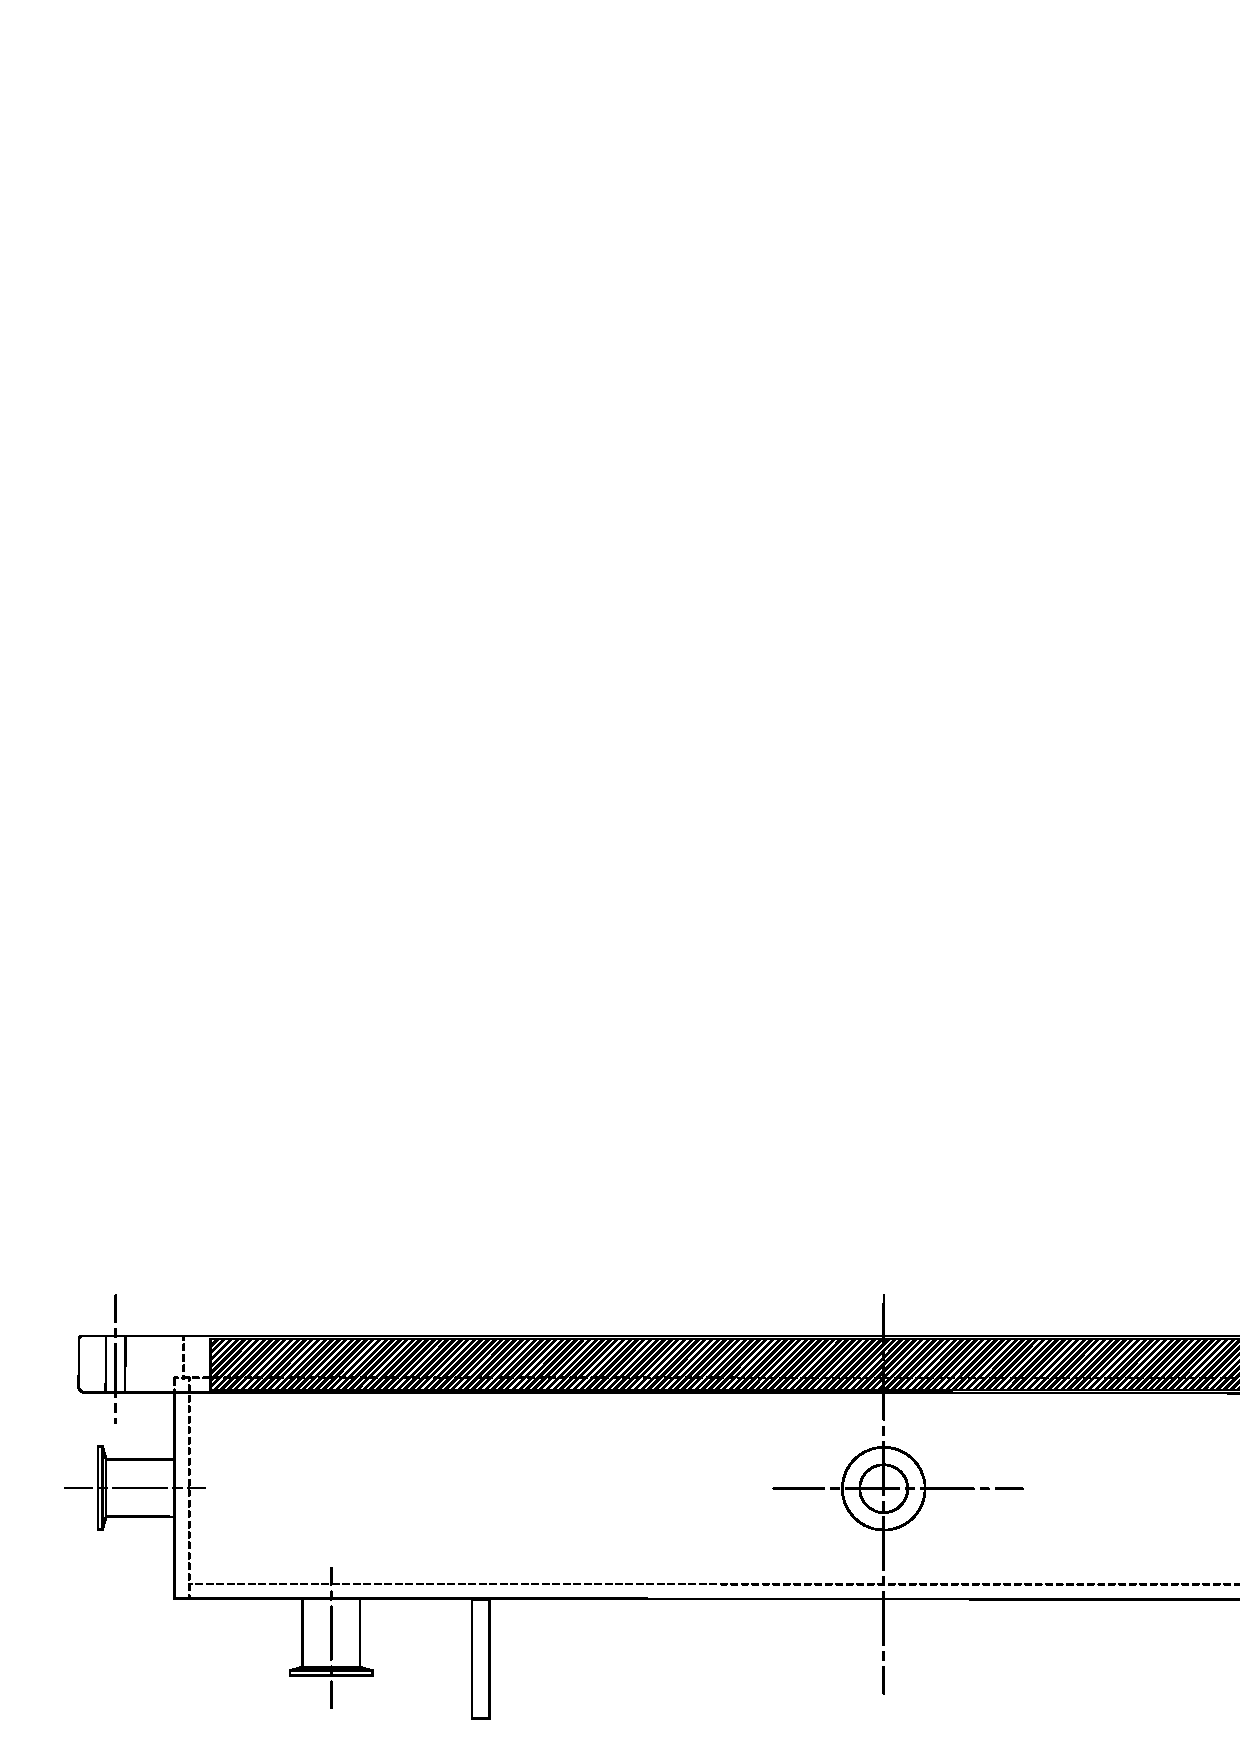
\includegraphics[width=6in]{figSOSwindow}
\caption{The SOS exit window and the vacuum test tank. \label{fig:sos_window}}
\end{figure}
\end{obsolete}

\infolevfour{
\paragraph{Window Material Testing}

Standard models used in predicting vacuum
window performance do not predict the actual performance of Kevlar laminate
fabrics accurately \cite{Mapes1993,Leonhardt,rllnl2}. Therefore, extensive tests of the
Mylar/Kevlar composite windows have been done and more are planned.
A summary of pressure
tests on windows composed of the custom laminated
fabric currently used in construction of all Hall~C vacuum windows is
given in Tables~\ref{tab:win_tst1} and \ref{tab:win_tst2}, below. Both vacuum and hydrostatic test 
tanks
are available for the HMS circular windows and for the SOS rectangular
window. Figure~\ref{fig:sos_window} shows a picture of the SOS vacuum
test tank.  The large round
HMS vacuum test tank uses the $8$ inch vacuum extension piece shown
earlier in Figure~\ref{fig:hms_window} (but removed from the spectrometer) with a $1.5$
inch thick aluminum blanking flange. For hydrostatic testing, windows (both
round and rectangular) are mounted directly on
blanking flanges with appropriate water fittings installed.

\begin{figure}
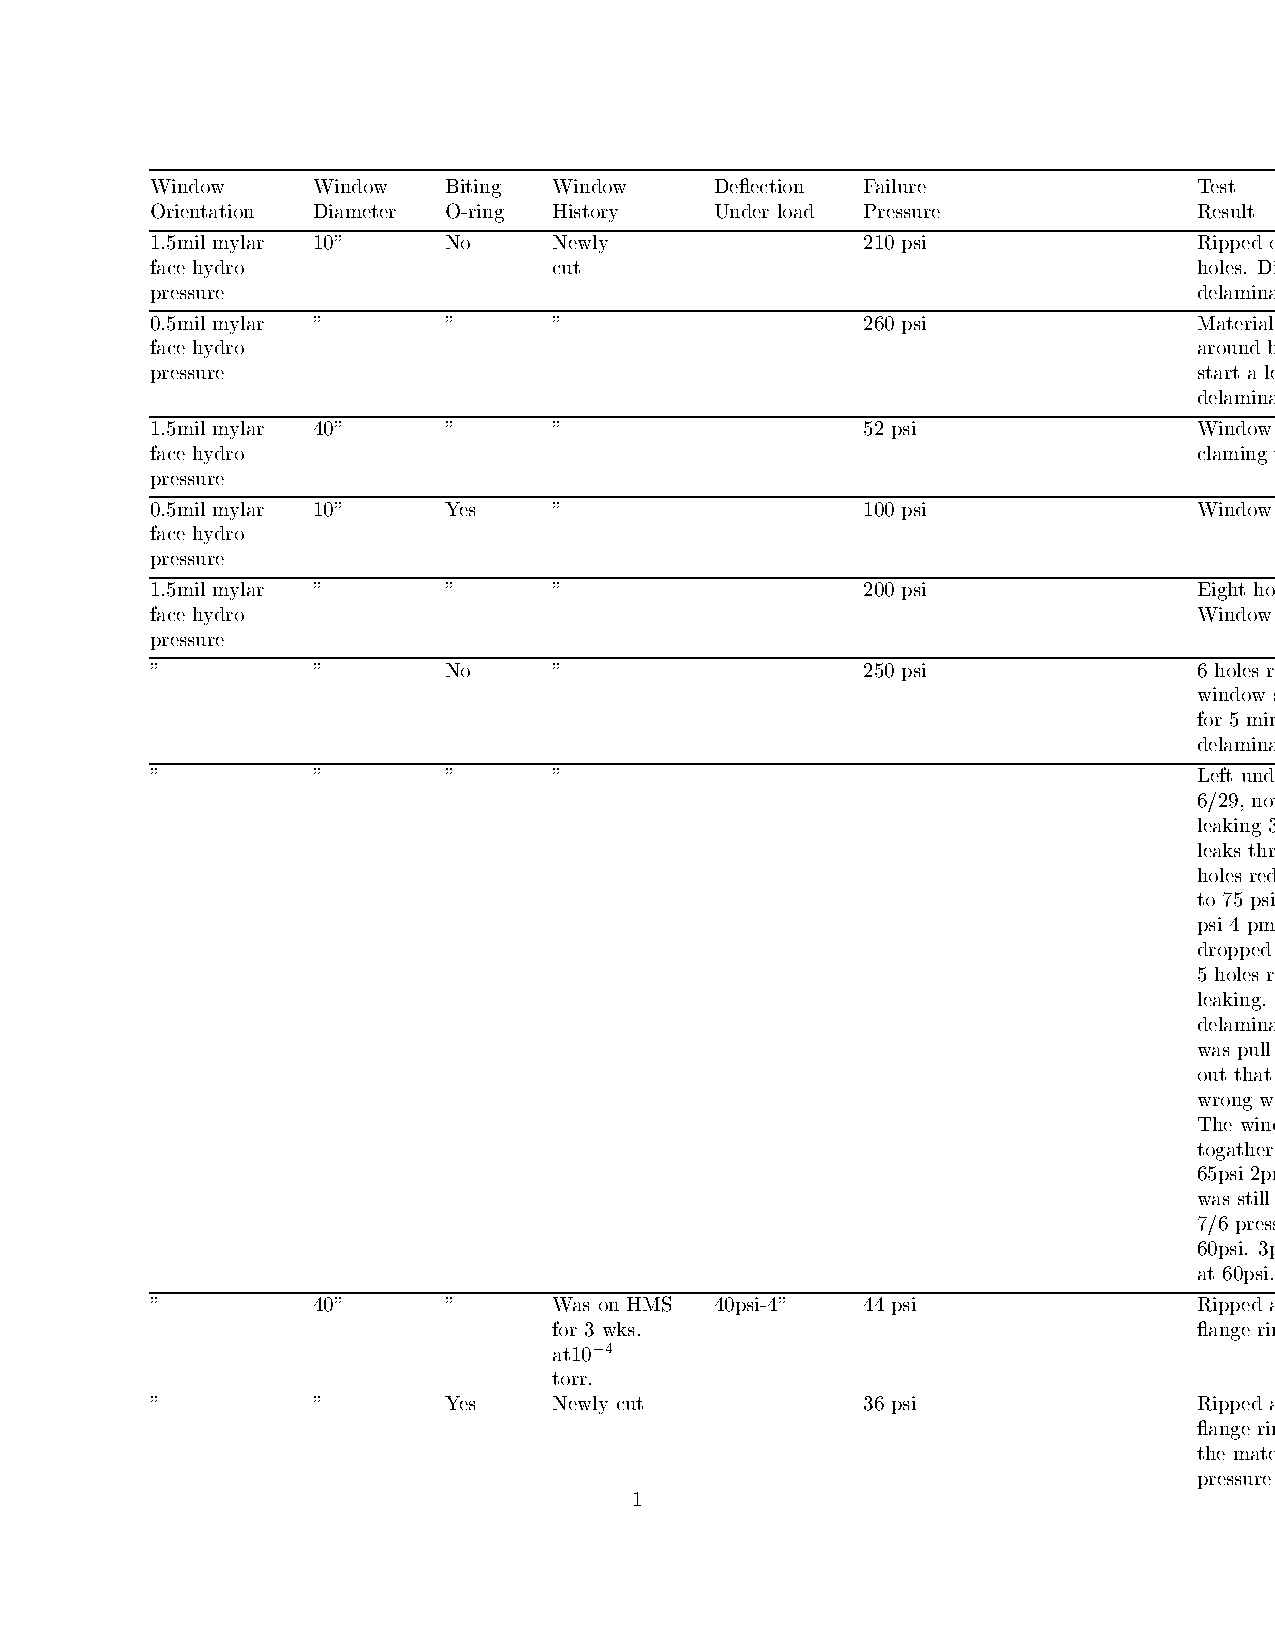
\includegraphics[height=7.5in]{vacuum}
\caption{Tests on the Hall~C Vacuum Windows (1 of 2) \label{tab:win_tst1}} 
\end{figure}
\clearpage

\begin{figure}
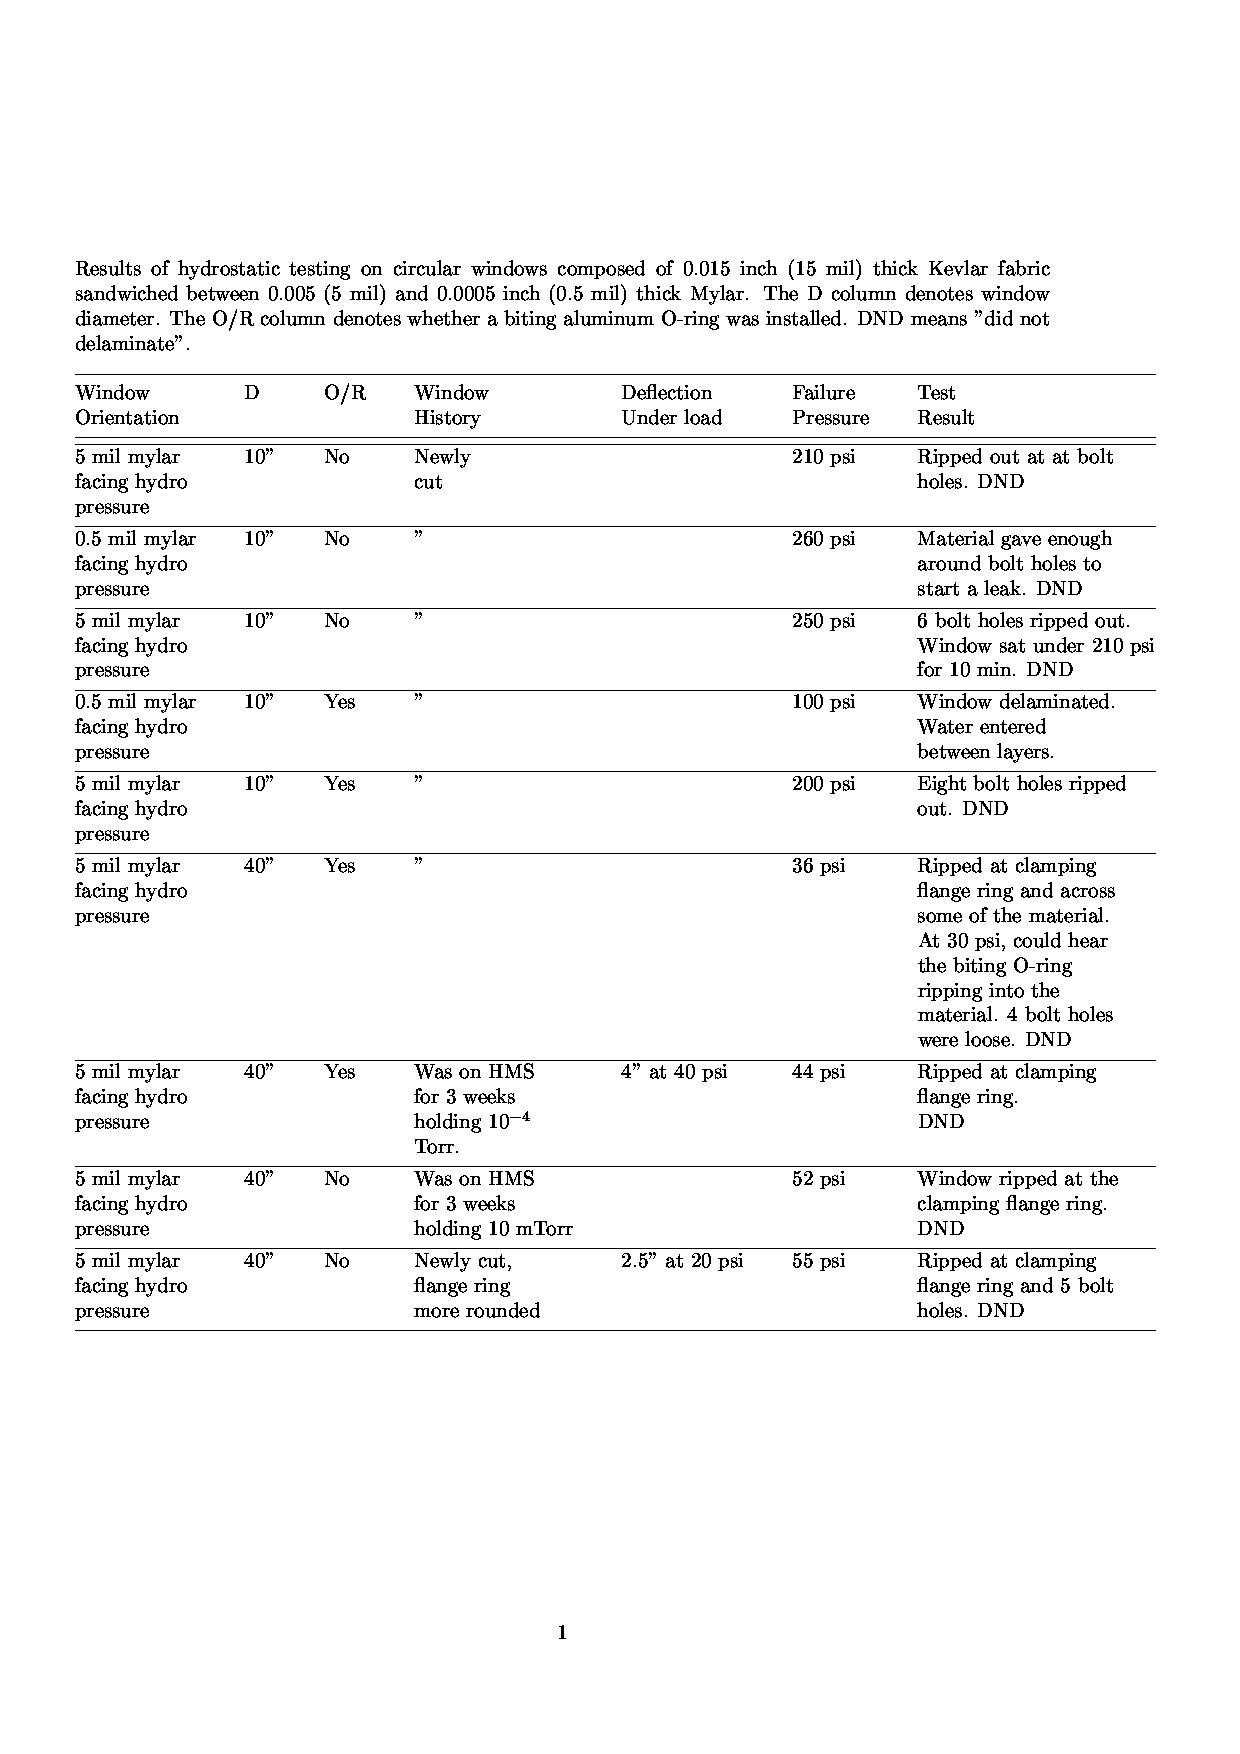
\includegraphics[height=7.5in]{vacuumc}
\caption{Tests on the Hall~C Vacuum Windows (2 of 2) \label{tab:win_tst2}}
\end{figure}
\clearpage

The tests show that the large HMS exit window does not begin to leak until
the pressure on it reaches over $3$ atmospheres. The small HMS window
did not begin to leak until over $14$ atmospheres of pressure was applied.
This is consistent with the load being transferred to
the outer circumference, the circumference of the small circle being four
times smaller than that of the large circle. The large rectangular SOS windows
began to leak at around 10 atmospheres. It may be possible to construct thinner
SOS vacuum windows for improved spectrometer resolution if required.

In addition to determining the absolute failure
pressure of the windows, a major goal of the testing effort was to
observe the failure modes of the
window material and flange design. The large windows failed by
ripping around the opening perimeter. The flange ring was then
rounded more and
a better result was obtained. It may be possible to further round the
flange if future tests indicate this to be necessary or advantageous.
The small windows failed by ripping out at the bolt holes.

Another question the tests in Table~\ref{tab:win_tst1} were designed to
answer was if
a biting aluminum clamping O-ring was necessary or advantageous. It was found
that windows with aluminum clamping rings failed at lower pressures than
windows without aluminum rings. The aluminum tended to tear the Mylar, allowing
leaking and uneven stress. The only window which delaminated had water between
the Mylar and Kevlar which leaked in through a tear in the
Mylar caused by the aluminum ring.

In conjunction with outlined full-size window testing, small samples
were subjected to stress and tensile analysis using strain gauge
instrumentation.  Through this work, it was found that the composite
window material maintained the Young's Modules of Kevlar, and had the
same ultinate failure load as Kevlar pieces of the same size.
Further, it was determined that the failure tears were along a
45$^{\circ}$ angle to the woven fibers, consistent with observations
of the rips in the destructively-tested full-size windows.  

In addition to the above testing efforts, two large round HMS exit windows
composed of the custom laminate material were ``knife" tested. The windows
were installed on the vacuum test tank and placed under vacuum. They were then
cut by a blade at the end of a long pole (so as to protect the personnel
testing the window from the results of a catastrophic failure). The window
did not rip any further than the cut and the
material did not delaminate. No evidence for catastrophic failure
was observed in either of these tests.

Although more long term reliability testing is necessary (see below),
results have so far been favorable.
Windows previously used on the HMS spectrometer are routinely hydro
tested to failure after biannual removeable and found to
hold up as well as freshly made windows (see, for example
Table~\ref{tab:win_tst1}).  Windows which have undergone multiple cycles fail at nearly the same pressure as uncycled
windows (see, for example, Table~\ref{tab:win_tst2}). A small round window did not fail after
being left pressurized for
a week at $65$ psi. (this test is not entered in the tables).
Entrance and exit windows composed of the Mylar/Kevlar laminate
material here described have held vacuum on the Hall C
spectrometer effectively and safely for over three years.


\paragraph{Vacuum Window Fabrication and Installation Procedure}

This procedure must be followed for installing any Hall~C spectrometer
vacuum window. One of the responsible personnel must be present during
all steps of fabrication and installation.
Although the procedure below is specifically for
the HMS large window, it is the same for the small HMS and for both SOS windows,
except as noted.
\begin{enumerate}
\item{Place window material, thin Mylar side down,
on a large flat, extremely clean, surface (such as
the marble table in EEL 126 after being washed).}

\item{Place window flange ring (also freshly cleaned) on top of material
and trace outer
circle (or rectangle for SOS) and bolt holes with transparency marking
pen.}

\item{Remove flange ring and cut out circle using Kevlar cutting 
shears.}

\item{Cut out bolt holes using appropriate (custom-made) drill press tool.
For the larger windows, this is a two person job as one is needed to hold the
material up so that it can't be nicked by the side of the drill press table
while the other concentrates on cutting the holes.}

\item{Clean the aluminum flange ring thoroughly and wipe with isopropyl
alcohol. For all but the HMS exit window, the flange ring and
window should be brought to the hall.  For the HMS exit window,
continue as outlined below from step 6 on.  For all other windows,
install flange ring and window unit to spectrometer vacuum flange
using standard O-ring vacuum seal practice (i.e. clean all surfaces
thoroughly with alcohol, apply vacuum grease, tighten in star pattern,
etc.)  All bolts should be torqued to 50 ft-lbs (40 ft-lbs for the
SOS exit window).  There must be a correctly tightened bolt in every
bolt hole.  Continue to step 17.}

\item{{\sl (HMS exit window)} Clean Viton O-ring with isopropyl alcohol and apply vacuum
grease as is standard for vacuum connections.}

\item{{\sl (HMS exit window)}Place Viton ring on HMS vacuum extension piece, composite
window over ring, and aluminum flange (clamping) ring over window.   Bolt together at four corners.}

\item{{\sl (HMS exit window)}Place and tighten bolts in a star pattern as appropriate for
standard O-ring vacuum seals.}

\item{{\sl (HMS exit window)}All bolts should be torqued to 50 ft-lbs (40 ft-lbs for the SOS
exit window).}

\item{{\sl (HMS exit window)}Using standard O-ring seal technique, mount other side of
vacuum extension piece on aluminum blanking flange.}

\item{{\sl (HMS exit window)}Using a transparency marker, trace the flange circle onto the
Mylar/Kevlar window.}

\item{{\sl (HMS exit window)}Begin vacuum pumping on extension
piece.} 

\item{{\sl (HMS exit window)}Note any creep of traced ring and window
deflection.  Check window for visual abnormalities or imperfections.}

\item{{\sl (HMS exit window)}Leave under vacuum for at least 1 hour.
Repeat step 13.}

\item{{\sl (HMS exit window)}Bring vacuum extension piece back to
atmospheric pressure and remove blanking flange.}

\item{{\sl (HMS exit window)}Being extremely careful not to touch the
Mylar/Kevlar window, install extension piece on HMS spectrometer in
hut using standard O-ring vacuum practice.}

\item{Clear detector hut and pivot area for initial pump down. Do not
allow entry for anyone other than the above named personnel to
these areas until a vacuum of at least 50 mTorr is achieved.}

\item{Begin vacuum pumping.}

\item{One of the above named personnel should check and note the
window deflections, recheck bolt torques, and generally look for
irregularities in the window deflections, before allowing
general entry to the detector
hut or pivot areas. That person should wear ear protection at all times while
near windows. Bolts should be retorqued if necessary.}

\item{Place a clearly visible tag near the vacuum window indicating
date of installation, estimated date of removal, and names and phone
numbers of contact personnel.}

\item{Recheck bolt torque, vacuum, and window deflection
again a couple of hours later (again, this should be done by
qualified personnel only, wearing hearing
protection). Retorque bolts if necessary.
If the window deflection has increased more than 3/4 inch, begin the entire
process again with a new window.}

\item{The windows should be changed as close to every 6 months as
reasonable given experiment run scheduling considerations. It is not
necessary to stop a run to change the windows, but they should be changed
as soon as possible thereafter.}

\end{enumerate}
} %infolevfour


%\paragraph{Safety Procedure for Working Near Vacuum Windows}

%Before entering the detector huts or pivot area, all personnel should check
%the spectrometer vacuum gauges. The HMS gauge is located under and near the Q3
%quadrupole. The SOS gauge hangs from the carriage beneath the quadrupole.
%Both gauges are monitored by video cameras and may be viewed
%in the counting house.
%If the spectrometers are under vacuum, the following procedure should be used.
%
%\begin{enumerate}
%\item{Before entering detector hut or pivot area, put on hearing
%protection. It is recommended that nobody should be
%closer than 3 feet from the windows without ear protection and that only
%those personnel who need to approach the windows be in their immediate
%vicinity.}
%
%\item{If entering HMS detector hut, close aluminum
%shutter over vacuum window before entering.}
%
%
%\item{If entering pivot area, check both spectrometer windows visually
%(from a distance greater than 3 feet if possible) for obvious wrinkles or
%discoloration. If any are observed, vacate area and
%contact one of the above named personnel. Never touch the vacuum 
%windows.}
%
%\item{Use careful judgement if it is necessary to work near the vacuum
%windows. Do not place objects so that they may fall on the windows, 
%etc.}
%
%\item{Do not work near the windows any longer than is absolutely
%necessary.}
%
%\item{Open aluminum
%HMS exit shutter only when all personnel have left the detector
%hut.}
%\end{enumerate}
%
%\paragraph{Vacuum Window Safety Summary}
%
%Catastrophic window failure would generate a significant shock wave as air
%rushed to fill the evacuated volume. It would make a loud noise which could
%damage the hearing of anyone standing close at hand at the time of failure.
%There are several indicators that something is wrong with the vacuum. If
%any of the following are observed, qualified personnel should be contacted
%and no one should approach the windows until one of those personnel have
%deemed it safe:
%
%
%
%\begin{enumerate}
%
%\item{Visual defects, particularly wrinkles, discoloration, or
%uneven fiber stress.}
%
%
%
%\item{Date of removal on tag near spectrometer window indicates
%a date near or after current date.}
%
%
%\item{Vacuum gauges indicating a loss of vacuum
%$\ge 1$ mTorr.}
%
%\item{HMS shutter malfunction (troubles opening or closing).}
%
%\item{The pen-traced ring drawn onto thae window perimeter moving away
%from the perimeter.}
%
%\item{Bolt torque not remaining at installed value
%(only qualified personnel should check for this).}
%
%\item{Deflection increasing above installed value
%(only qualified personnel should check for this).}
%\end{enumerate}
%





